\section{System Architecture}

The \textbf{RoadSense} consists of multiple IoT devices installed in vehicles, communicating with a central server designed to be highly scalable to handle data from thousands of devices. In this section we will describe all meaningful components of the system, focusing on the IoT data pipeline and the client-server architecture.

\subsection{IoT Data Pipeline}

The data pipeline has been designed with scalability in mind, allowing for efficient data collection, processing, and data analysis from multiple (potentially thousands) concurrent IoT devices. The following diagram illustrates the pipeline steps, from data ingestion to the storage of processed data.

\begin{figure}[H]
	\centering
	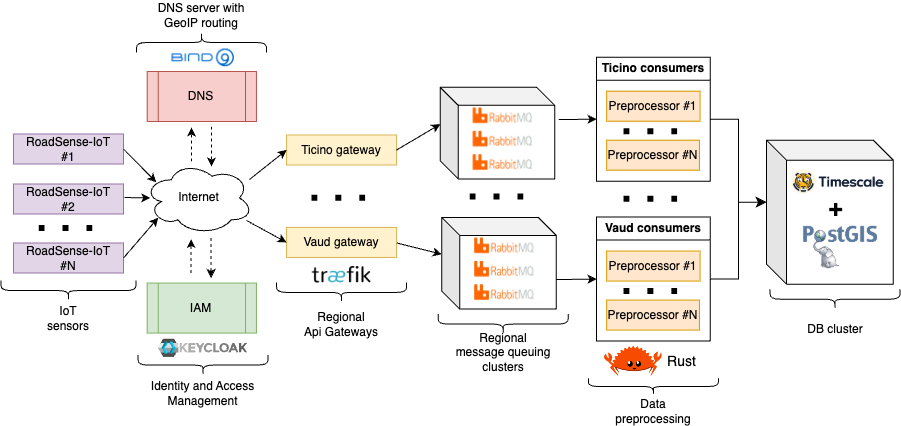
\includegraphics[width=\textwidth]{../../assets/diagrams/iot_data_pipeline/iot_data_pipeline.png}
	\caption{IoT Data Pipeline}
\end{figure}

The pipeline consists of the following components:

\begin{enumerate}
	\item \textbf{Data ingestion}: IoT devices collect vibration, GPS, and other relevant data points. When the vehicle reaches an access point, the data will be transmitted to the server. Each device will be able to connect to different Wi-Fi networks, allowing for data transmission in different locations. This may include public Wi-Fi networks, cellular data, or a dedicated network infrastructure.

	\item \textbf{Authentication and security}: In the original idea of the project each device is authenticated before data transmission to ensure data integrity and prevent unauthorized access. For this purpose, was decided to use \href{https://www.keycloak.org/}{Keycloak} for identity and access management. Unfortunately, this feature was not implemented in the presented prototype in order to focus on the core functionality of the system.

	\item \textbf{Geographical distribution}: The server leverages DNS-based load balancing to distribute incoming data across regional gateways for efficient processing. We have chosen to use \href{https://www.isc.org/bind/}{BIND9} for DNS-based load balancing along with \href{https://www.maxmind.com/en/geoip2-databases}{GeoIP} for geolocation. Each regional gateway will be responsible for routing the user requests to the regional message queuing system. For this purpose, we will use \href{https://traefik.io/}{Traefik} as the reverse proxy. Unfortunately, also this feature was not implemented in the prototype as it would introduce additional complexity to the system. However, this feature is essential for the scalability of the system as it allows for efficient data processing across multiple regions.

	\item \textbf{Message queues}: Each gateway node processes incoming data and forwards it to a regional queuing system to allow for parallel processing. After evaluating multiple options, we decided to use \href{https://www.rabbitmq.com/}{RabbitMQ} as the message queue system. To ensure high availability, we will deploy RabbitMQ in a cluster configuration (refer to the \href{https://www.rabbitmq.com/clustering.html}{RabbitMQ Clustering Guide}). For the prototype we avoided the creation of a RabbitMQ cluster, and was used a single instance of RabbitMQ. This feature is still of interest for the scalability of the system.

	\item \textbf{Data preprocessing}: Each region has a set of preprocessing microservices that consume incoming data from the regional message queuing system, perform data validation, and run initial data processing tasks. These microservices are deployed using containerization technology like Docker and in a future production environment, managed by \href{https://kubernetes.io/}{Kubernetes}.
	      During the initial specification of the project was decided to use \href{https://golang.org/}{Go} as the primary language for these microservices. However, in the prototype was used \href{https://rust-lang.org/}{Rust} as the primary language for the microservices. This choice was made to explore the performance and safety features of Rust. The microservices were designed to be lightweight, efficient and fail-safe.

	\item \textbf{Data storage}: Processed data is stored in a scalable database system that can handle high volumes of data. Since we are dealing with both date-time and geospatial data, we chose to use \href{https://www.timescale.com/}{TimescaleDB} as the database system with the \href{https://postgis.net/}{PostGIS} extension to support geospatial queries.
	      PostGIS was used to store and query collected samples
\end{enumerate}

\subsection{Client-Server Architecture}

This section describes the client-server architecture of the system, focusing on the interaction between the web application and the server-side components. The following diagram illustrates how the client (web browser) interacts with the server to load and visualize collected data:

\begin{figure}[h!]
	\centering
	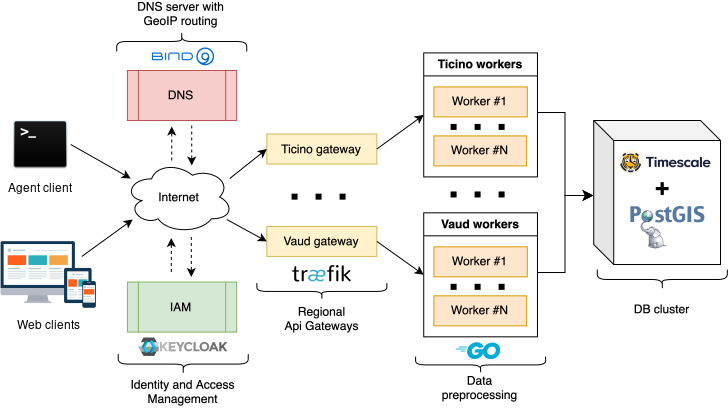
\includegraphics[width=0.5\textwidth]{../../assets/diagrams/web_app_architecture/web_app_architecture.png}
	\caption{Client-Server Architecture}
\end{figure}

The pipeline consists of the following components:

\begin{enumerate}
	\item \textbf{Clients}: The application users (agents or web browsers) interact with the web application to view road conditions, manage alerts, and access other features.
	\item \textbf{Authentication}: To manage user access and permissions, users need to authenticate themselves. For this purpose, we will use the same instance of \href{https://www.keycloak.org/}{Keycloak} that is used for IoT device authentication. To have a greater division between IoT devices and users, we will employ different realms in Keycloak (refer to the \href{https://www.keycloak.org/docs/latest/server_admin/index.html#core-concepts-and-terms}{Keycloak Documentation}).
	\item \textbf{Geographical distribution}: API requests are routed to the regional API gateways using DNS-based load balancing. We will use the same \href{https://www.isc.org/bind/}{BIND9} + \href{https://www.maxmind.com/en/geoip2-databases}{GeoIP} + \href{https://traefik.io/}{Traefik} setup as described in the IoT data pipeline section.
	\item \textbf{API Workers}: Each region has a set of API worker microservices that will handle incoming API requests, query the database, and return the requested data to the client. These microservices will be deployed using containerization technology like Docker and managed by \href{https://kubernetes.io/}{Kubernetes} in a future production environment. Furthermore, they will be developed using \href{https://golang.org/}{Go} to enhance the application performance.
	\item \textbf{Database cluster}: API workers connect to the database cluster containing the aggregated IoT data, allowing them to retrieve the necessary information for the client requests.
\end{enumerate}
